\section{Discussion}
\label{sec:discussion}

% In this section we discuss how the idea of auxiliary histories, which
% can store observed thread interference, can be applied to reason
% quantitatively about other non-linearizable concurrent structures.
%

% \paragraph{Balancer-based concurrent container implementations}

{
\setlength{\belowcaptionskip}{-10pt}
\begin{figure}
\centering
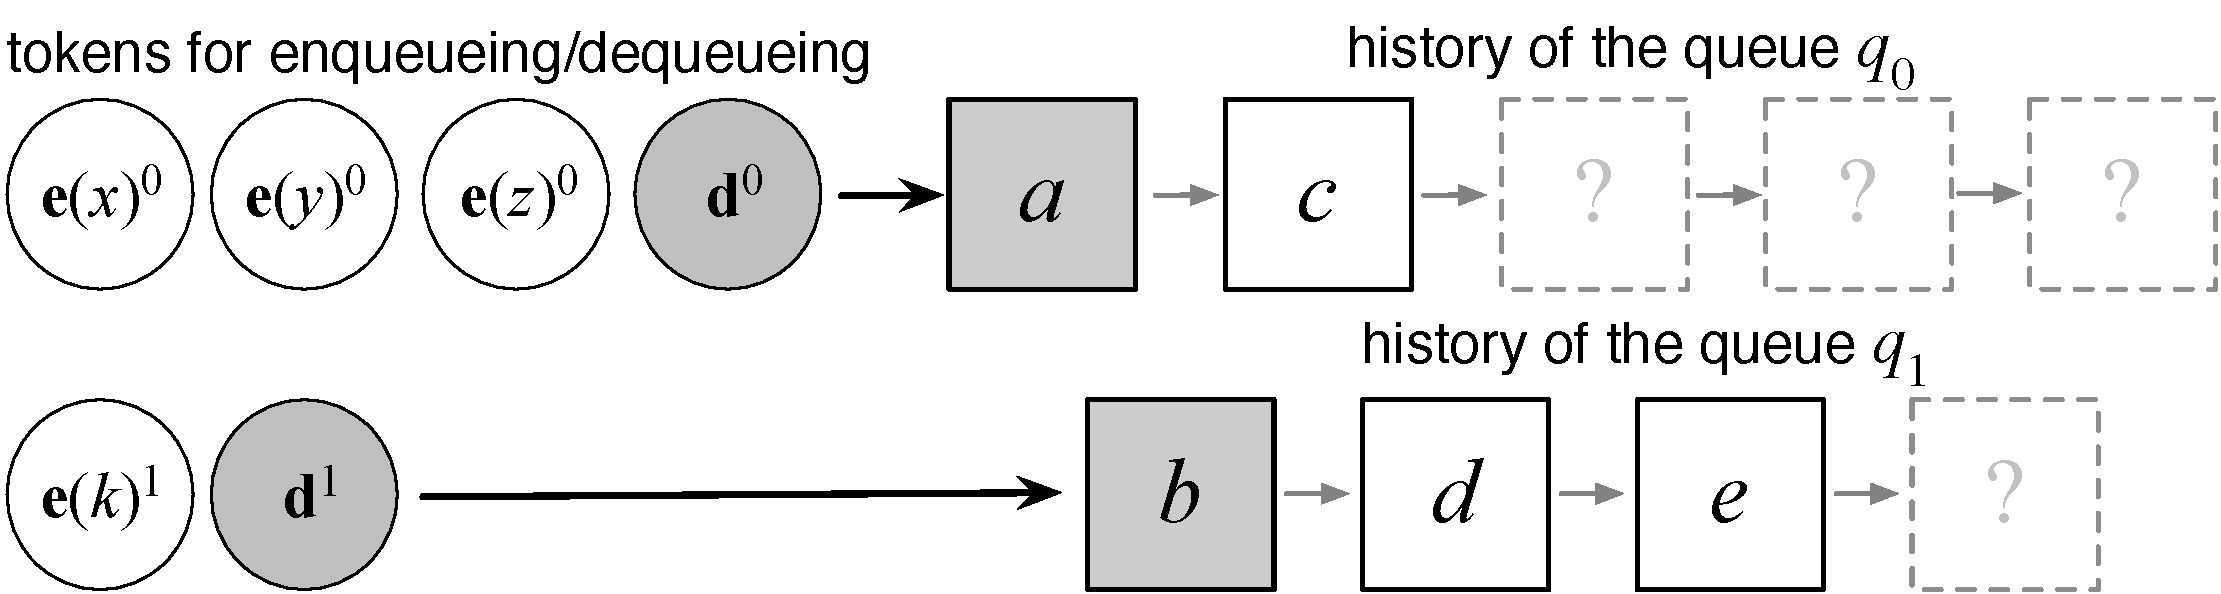
\includegraphics[width=8.2cm]{chist2.pdf}      
\caption{Tokens and histories of a balancer-based queue.}
\label{fig:chist2}
\end{figure}
}

% In Section~\ref{sec:counting}, we have shown how one can reason
% quantitatively about behavior of a counting network, implemented via a
% balancer, using histories, whose entries snapshot interference,
% therefore characterizing the out-of-order discrepancies between its
% results.

%
\begin{wrapfigure}[8]{r,trim}[-45pt]{1.5cm}   
\centering 
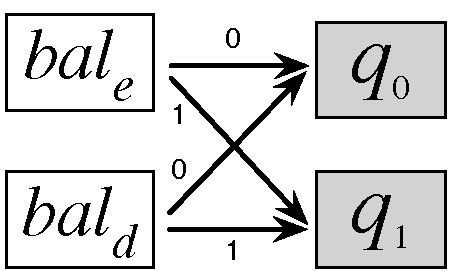
\includegraphics[width=3.0cm]{queue.pdf} 
\end{wrapfigure}
%
The idea of interference-capturing histories, which allowed us to
characterize the out-of-order discrepancies between the results of a
counting network in Section~\ref{sec:counting},
%
can be applied to provide specifications for other
balancer-based data structures, for instance,
queues~\cite{Derrick-al:FM14} and
stacks~\cite{Jagadeesan-Riely:ICALP14}.
%
The picture on the right illustrates schematically a non-linearizable
queue~\cite{Derrick-al:FM14}, which is built out of two \emph{atomic}
queues, $q_0$ and $q_1$, and two balancers, $\bal_e$ and $\bal_d$.
The balancers are used to distribute the workload between the two
queues by directing the threads willing to enqueue and dequeue
elements, correspondingly.

%Taking inspiration from the development in Section~\ref{sec:counting},
%
One can think of representing the pending enqueue/dequeue requests to
each of the two queues, $q_0$ and $q_1$, by two separate sets of
tokens, as shown in Figure~\ref{fig:chist2}.
%
The white and gray boxes correspond to the present and
dequeued nodes in the queue in the order they were added/removed.
%
Therefore, white elements are those that are currently in the queue.
%
Similarly, the white-colored tokens are for enqueueing elements, so
the elements $x$, $y$, $z$ and $k$ are going to be added to the
corresponding atomic queues. Gray-colored tokens correspond to
dequeueing capabilities for one or another atomic queue, distributed
among the threads, so the elements $c$ and $d$ are going to be removed
next, on the expense of the corresponding dequeue tokens.
%
The timestamps of the entries in the queue history, omitted from the
figure, are created, as elements are being enqueued to $q_0$ and
$q_1$, and the parity of a timestamp corresponds to the atomic queue
being changed. Thus, there might be ``gaps'' in the combined queue
history reminiscent to the gaps in the counter history from
Section~\ref{sec:counting} (\eg, the gap caused by the absence of an
``even'' element in the combined history right between $d$ and $e$ in
Figure~\ref{fig:chist2}, as indicated by ``?''), which will cause
out-of-order anomalies during concurrent executions.
%
%
By accounting for the number of past and present tokens for enqueueing
and dequeueing, one should be able to capture the effects of
interference and express a quantitative boundary on the discrepancy
between the results, coming out of order, in terms of ordering of
timestamps, assigned to enqueue/dequeue events in the combined queue
history.

The intuition is similar in the case of balancer-based
stacks~\cite{Jagadeesan-Riely:ICALP14}, with the main difference being
that the elements are removed in a LIFO order and, hence, the
\emph{rightmost} entries of a corresponding partial (\ie, even or odd)
history are painted gray first.
%
We leave complete formalization of these structures to the future
work.




% \paragraph{Counting networks with arbitrary width}

% For the sake of simplicity, when presenting the main ideas of
% interference-capturing histories in Section~\ref{sec:counting}, we
% assumed that the balancer can return only 0 and 1.
% %
% However, the development of a counting network and the balancer-based
% structures, described previously, can be directly generalized for
% networks of arbitrary width $W$, not just 2.

% In particular, assuming that the balancer's return values are
% $0, 1, \ldots$ modulo $W$, the invariant~\ref{cn:ai} in
% Section~\ref{sec:count-netw-invar} will have to be changed, so all
% $2$'s in it are replaced by the value of $W$, and the history entries
% will be storing $W$ projections from the interference (\ie,
% $\tknh^0, \ldots, \tknh^{W-1}$) instead of just $\tknh^0$ and $\tknh^1$.
% %
% Similarly, the inequalities in the final specification of
% \code{getAndInc}~\eqref{eq:qc-spec}, will have to use $W$ instead of 2
% as a summand and factor for bounding the discrepancy caused by the
% interference, which in its turn will be expressed via the sum
% $\sum_{i = 0}^{W - 1}|\iknh^i \cap \ikno^i|$.

% \todo{Explain, what would need to be changed in our formalization in
%   Section~\ref{sec:counting} if we consider a network with the width
%   $W$.}.

% \paragraph{An alternative design of histories for counting networks}

% While the definitions of the simple counting network's auxiliary state
% and protocol, described in Section~\ref{sec:counting}, suffice to
% establish the spec, which bears all desired properties, other designs
% choices were possible, basing on the same idea of
% \emph{interference-capturing histories}.

% For instance, instead of storing tokens, representing interfering
% threads, in history entries of the form
% $t \hpts (\tknh^0, \tknh^1, z)$, we could have stored the events of
% getting/spending tokens as separater entries, $t \hpts \mathsf{Got}~z$
% and $t \hpts \mathsf{Spent}~z$, in addition to entries, corresponding
% to incrementing a counter $c_b$, $t \hpts \mathsf{Inc}~b~v$. In such
% representation, history timestamps would correspond to logical moments
% of time, instead of counter values, and the state invariants would be
% relating the values of the two counters to the sets of even and odd
% tokens, which are ``alive'' and ``dead'', inferred from the history up
% to date. This would allow us to embed the
% predicate~$\happrox$~\eqref{eq:happrox} directly to the state
% invariant and not mention it in the spec~\eqref{eq:qc-spec},
% therefore, giving us a shorter specification of \code{getAndInc} on
% the expense of more complicated state/history resource invariants.

